\begin{figure}
    \centering
    \subfigure[\label{buch:papers:Wirbelringe:fig:versuch_moment_1}]{
        %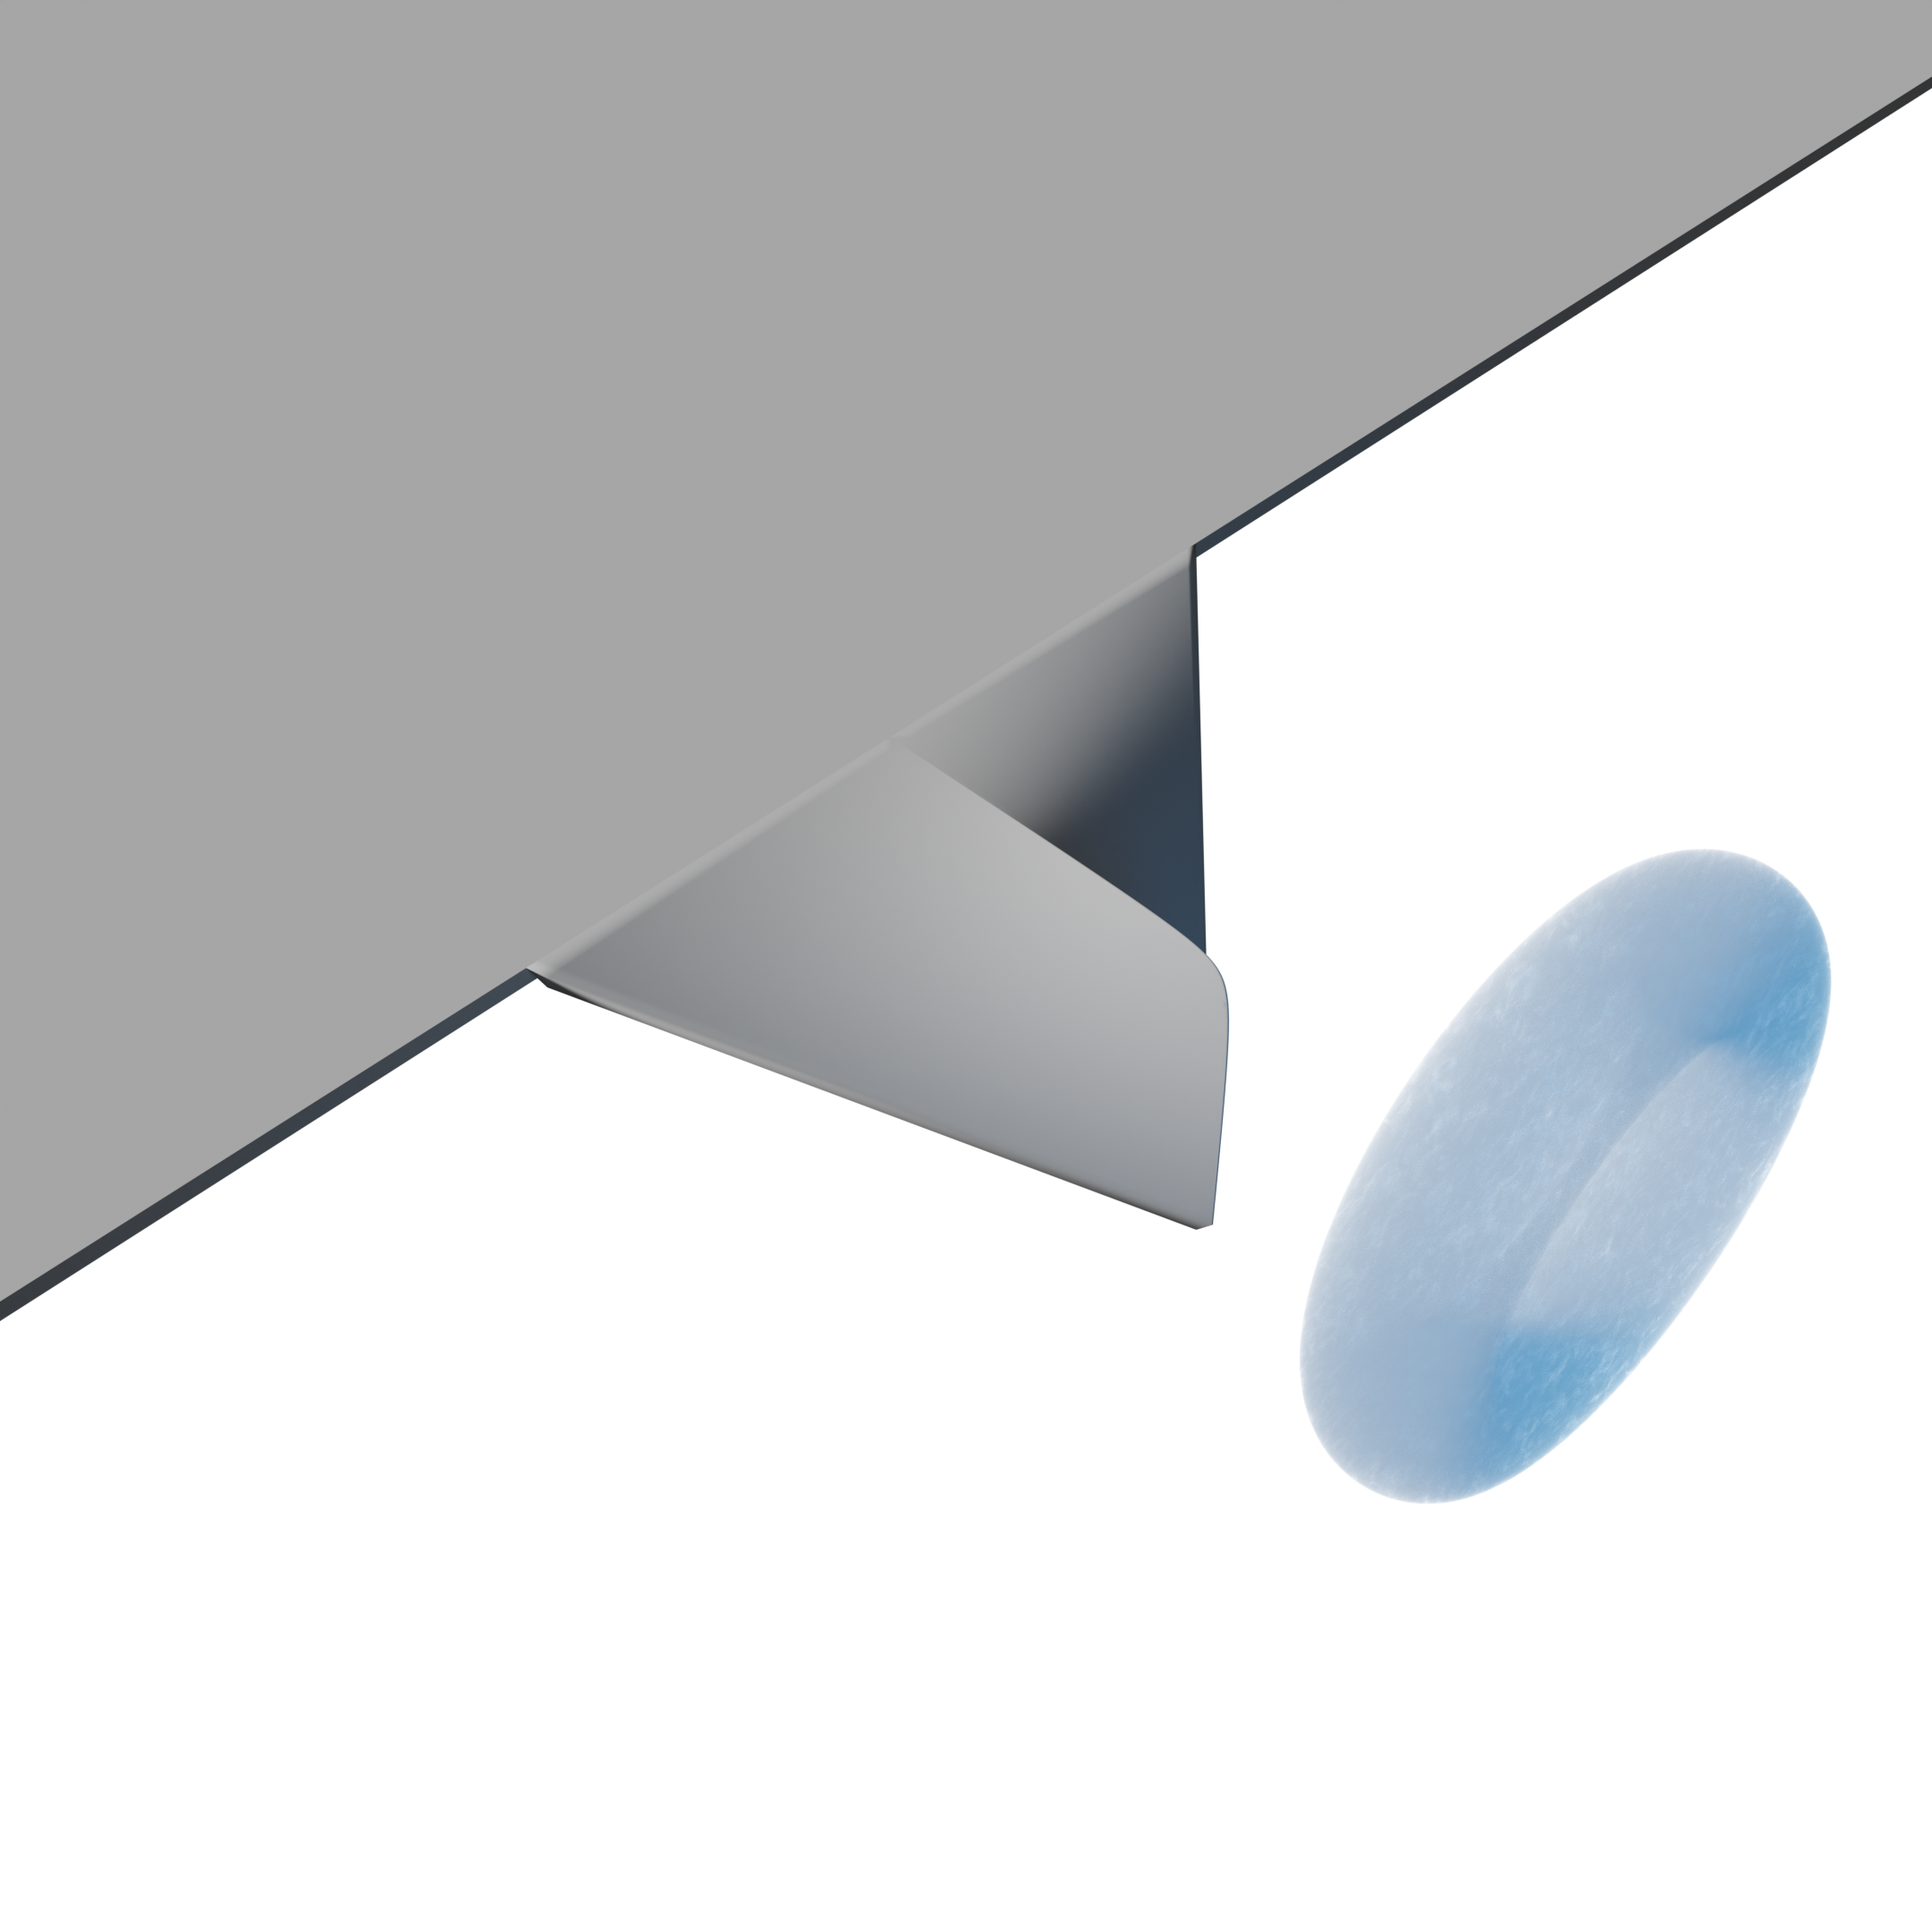
\includegraphics[width=0.3\textwidth]{papers/wirbelringe/fig/versuch_moment_1.png}
        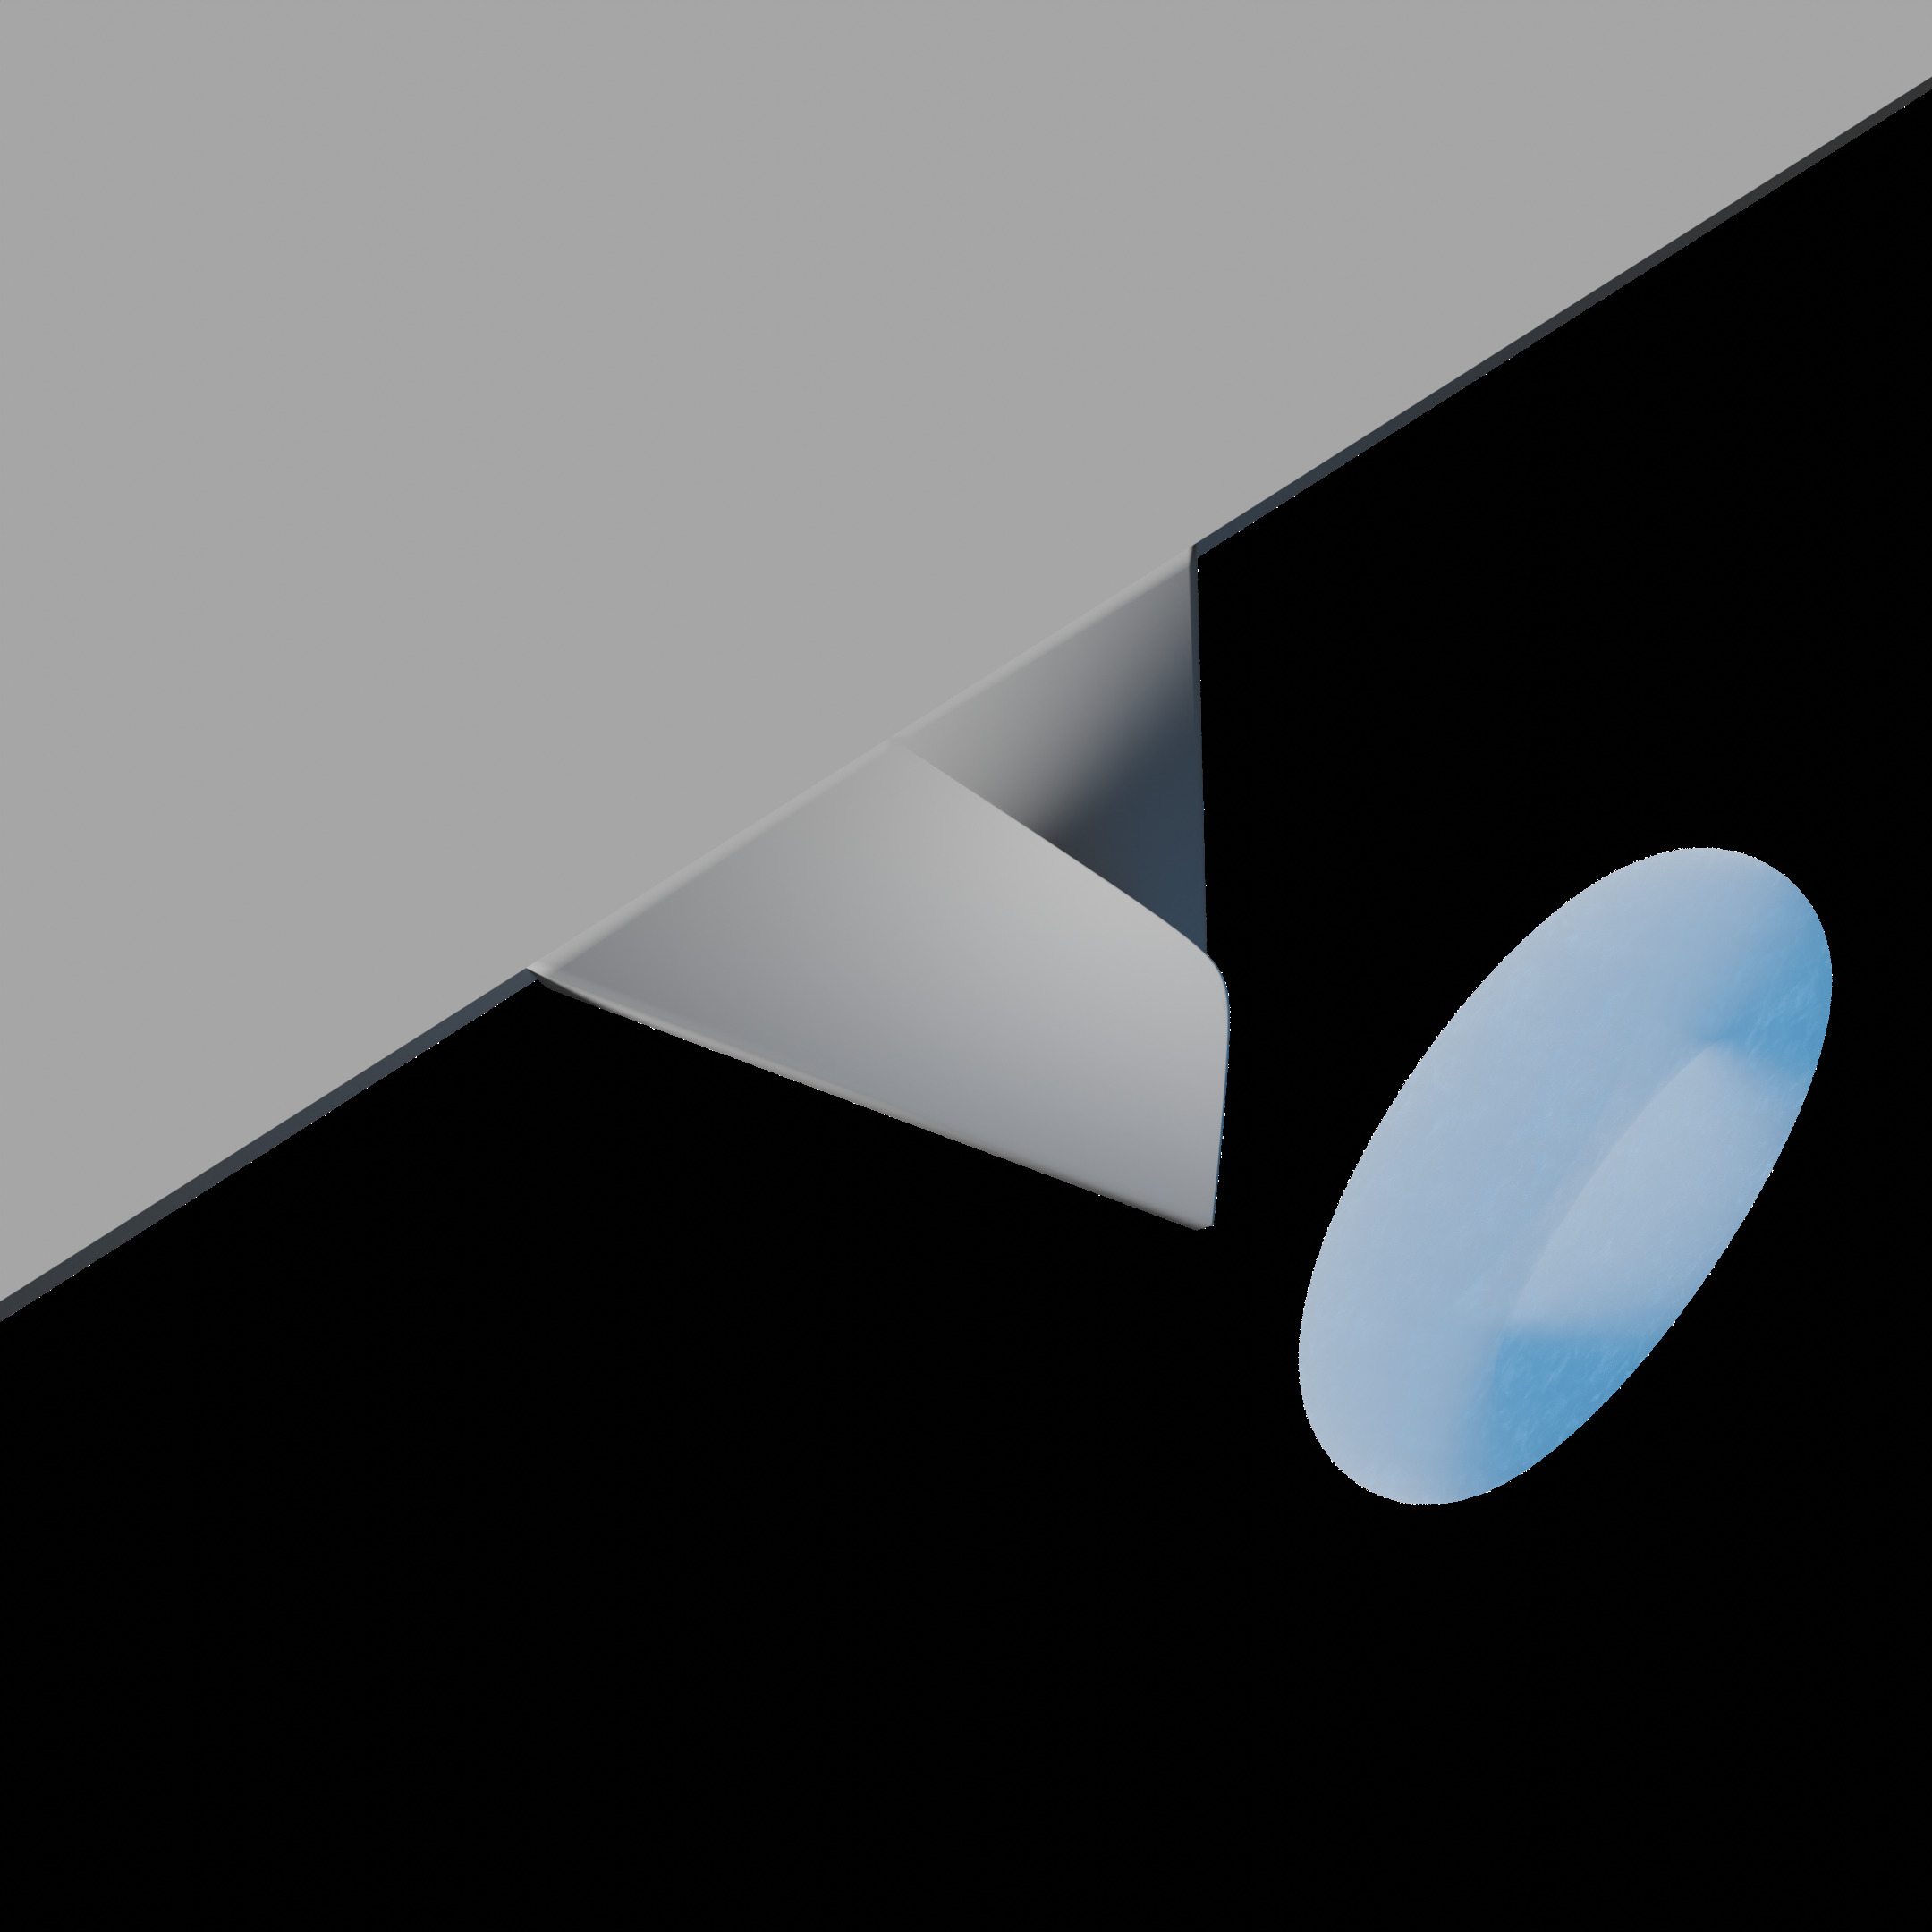
\includegraphics[width=0.3\textwidth]{papers/wirbelringe/fig/versuch_moment_1.jpg}
    }\hfill
    \subfigure[\label{buch:papers:Wirbelringe:fig:versuch_moment_2}]{
        %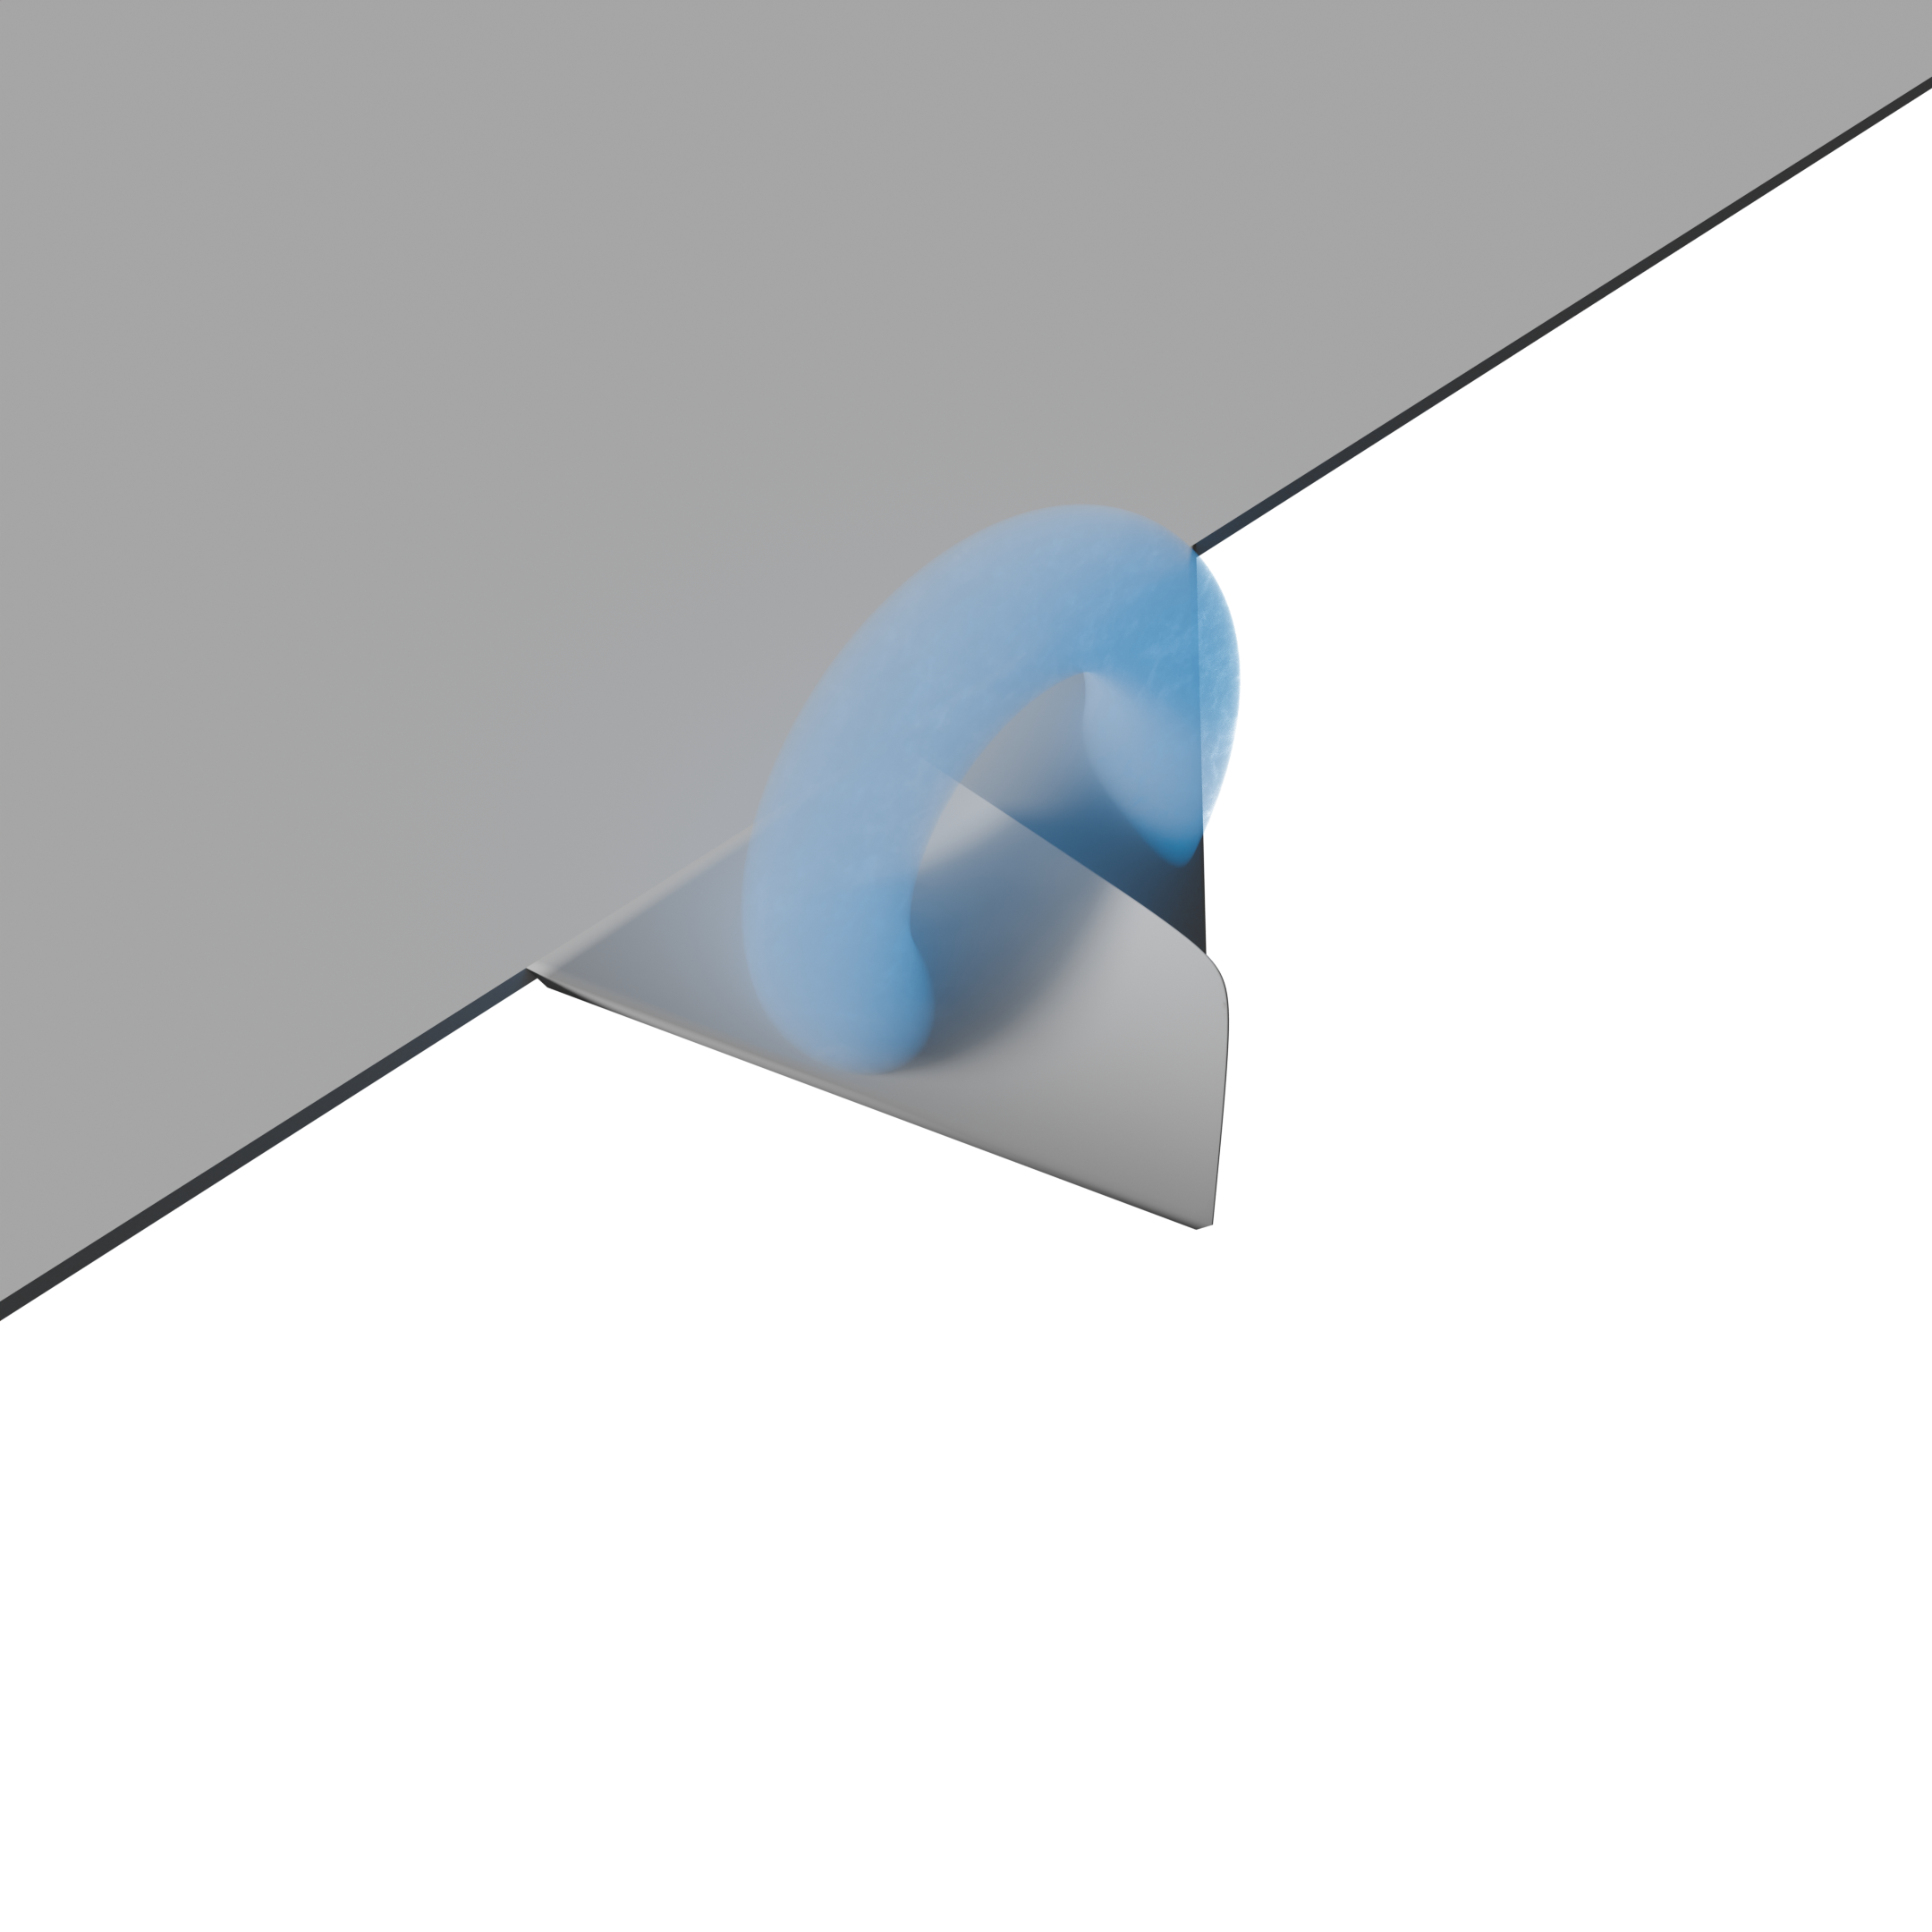
\includegraphics[width=0.3\textwidth]{papers/wirbelringe/fig/versuch_moment_2.png}
        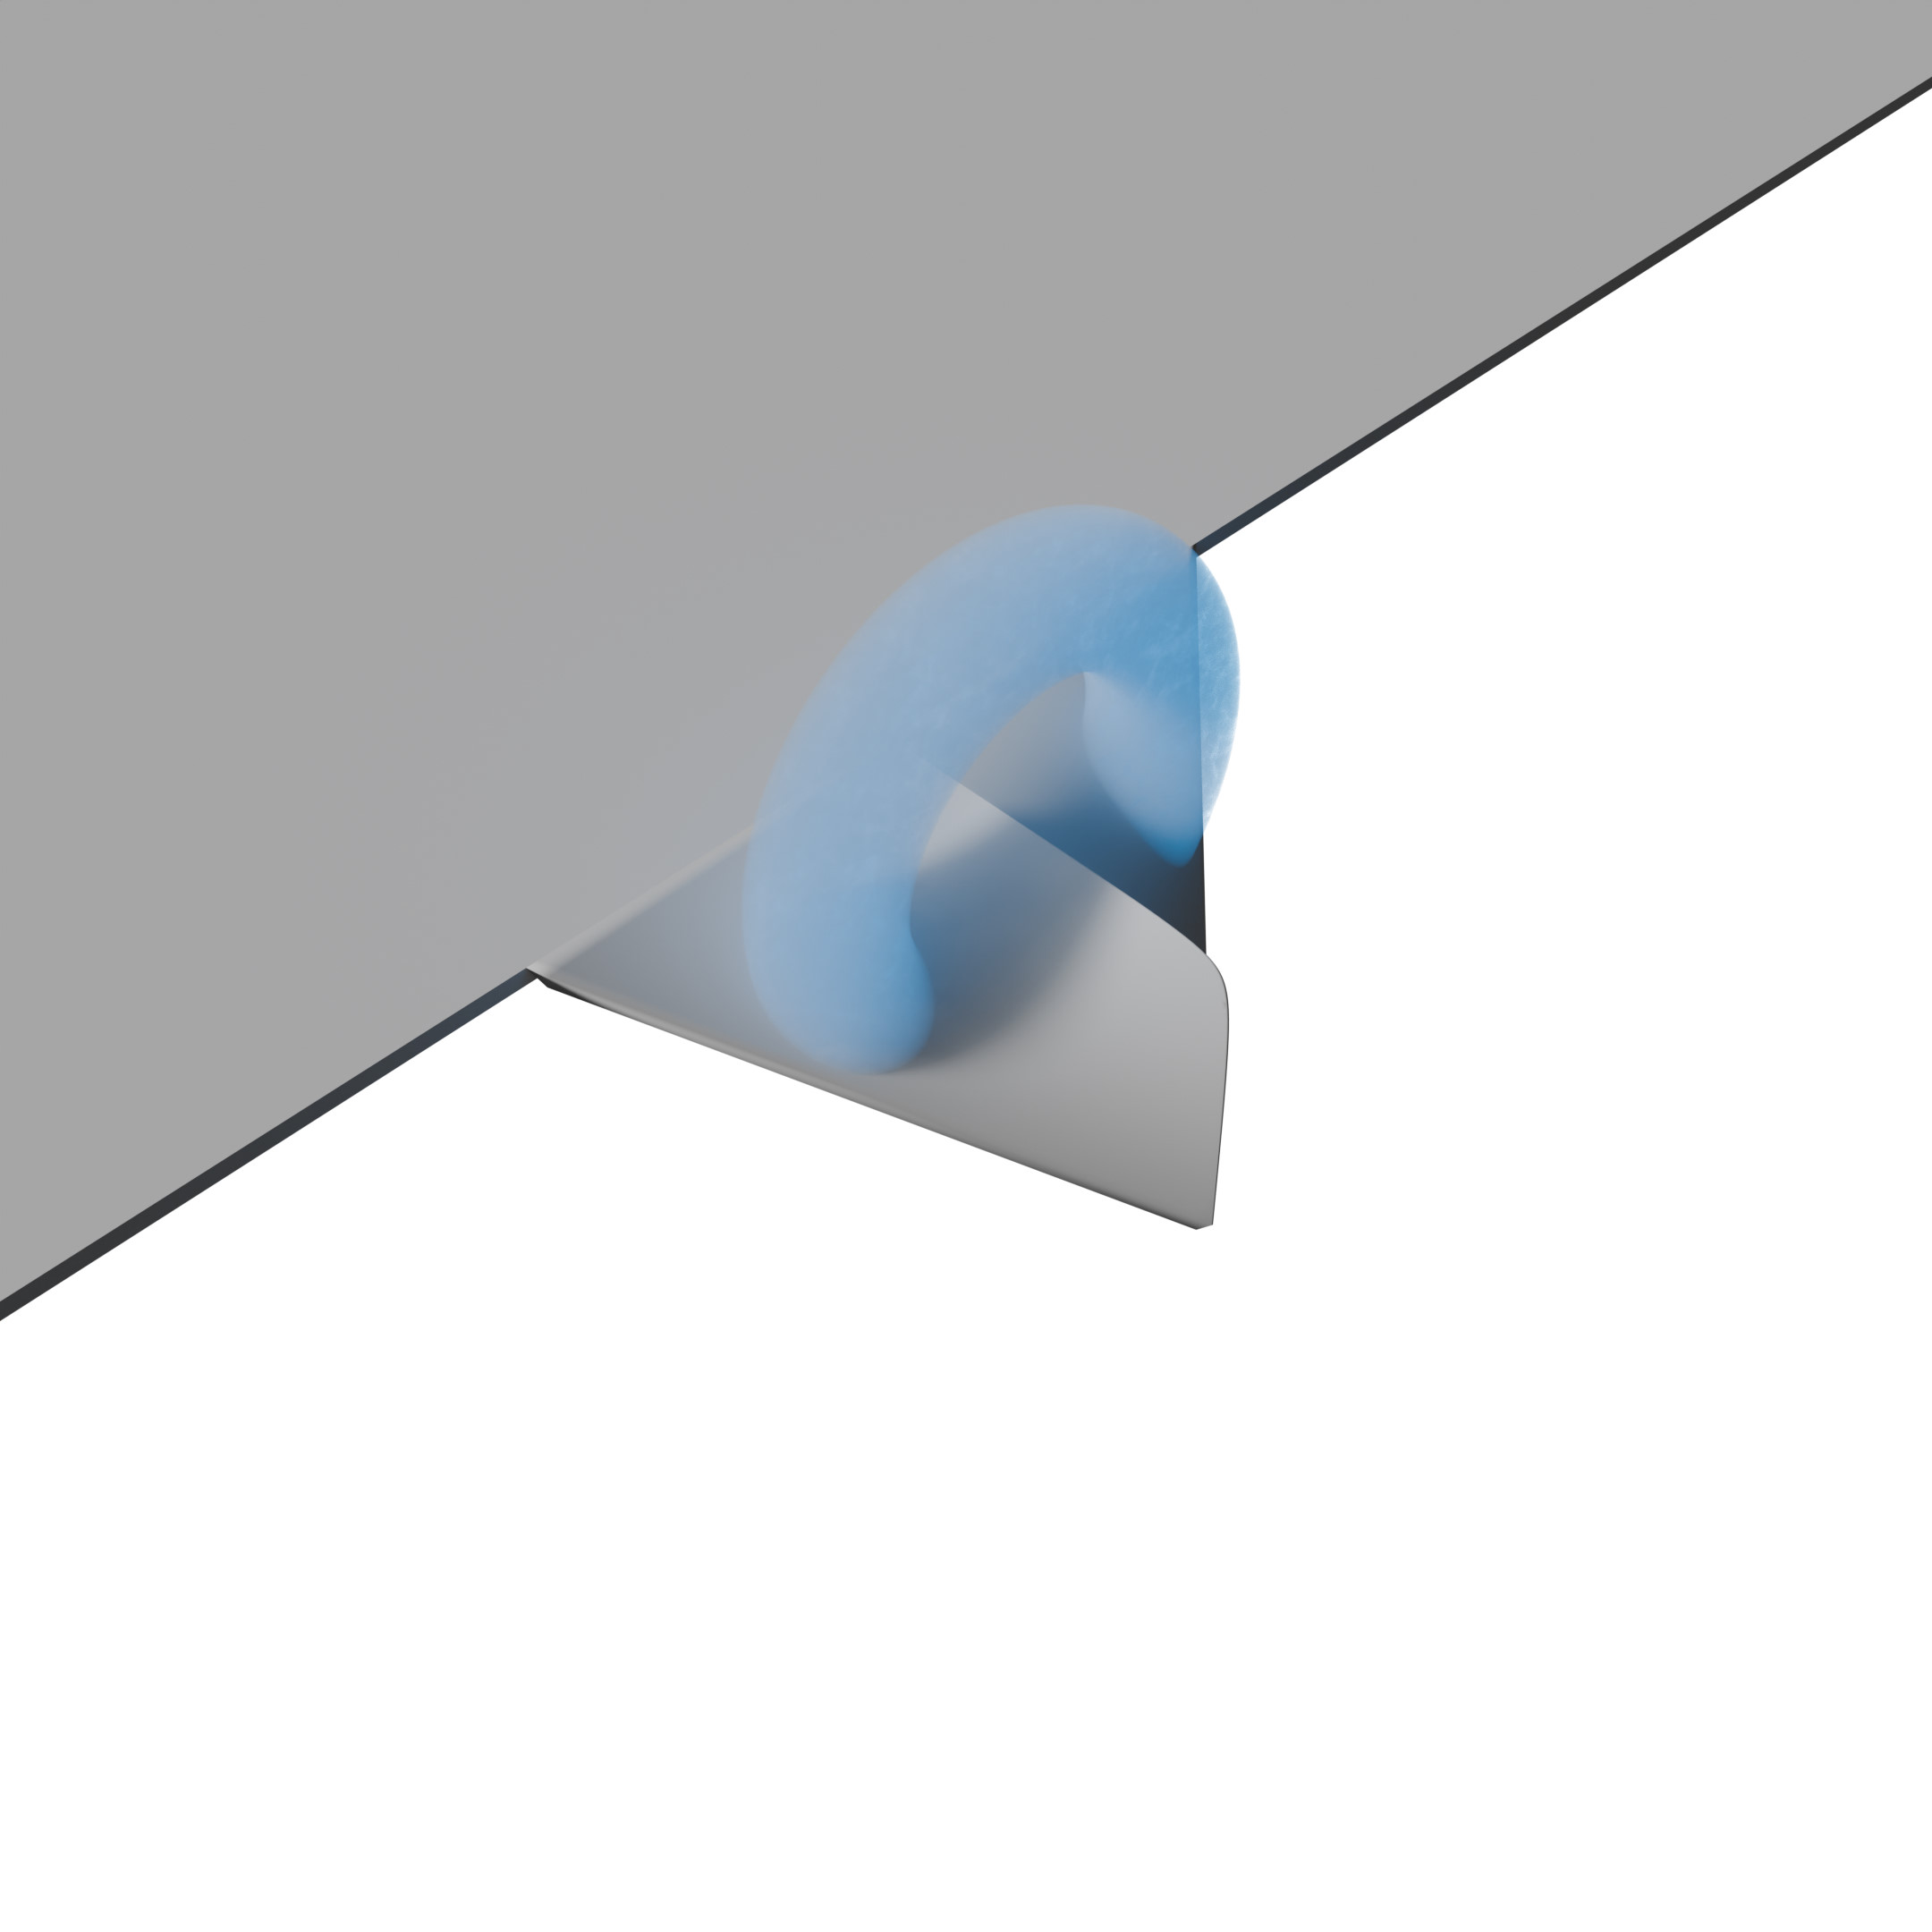
\includegraphics[width=0.3\textwidth]{papers/wirbelringe/fig/versuch_moment_2.jpg}
    }\hfill
    \subfigure[\label{buch:papers:Wirbelringe:fig:versuch_moment_3}]{
        %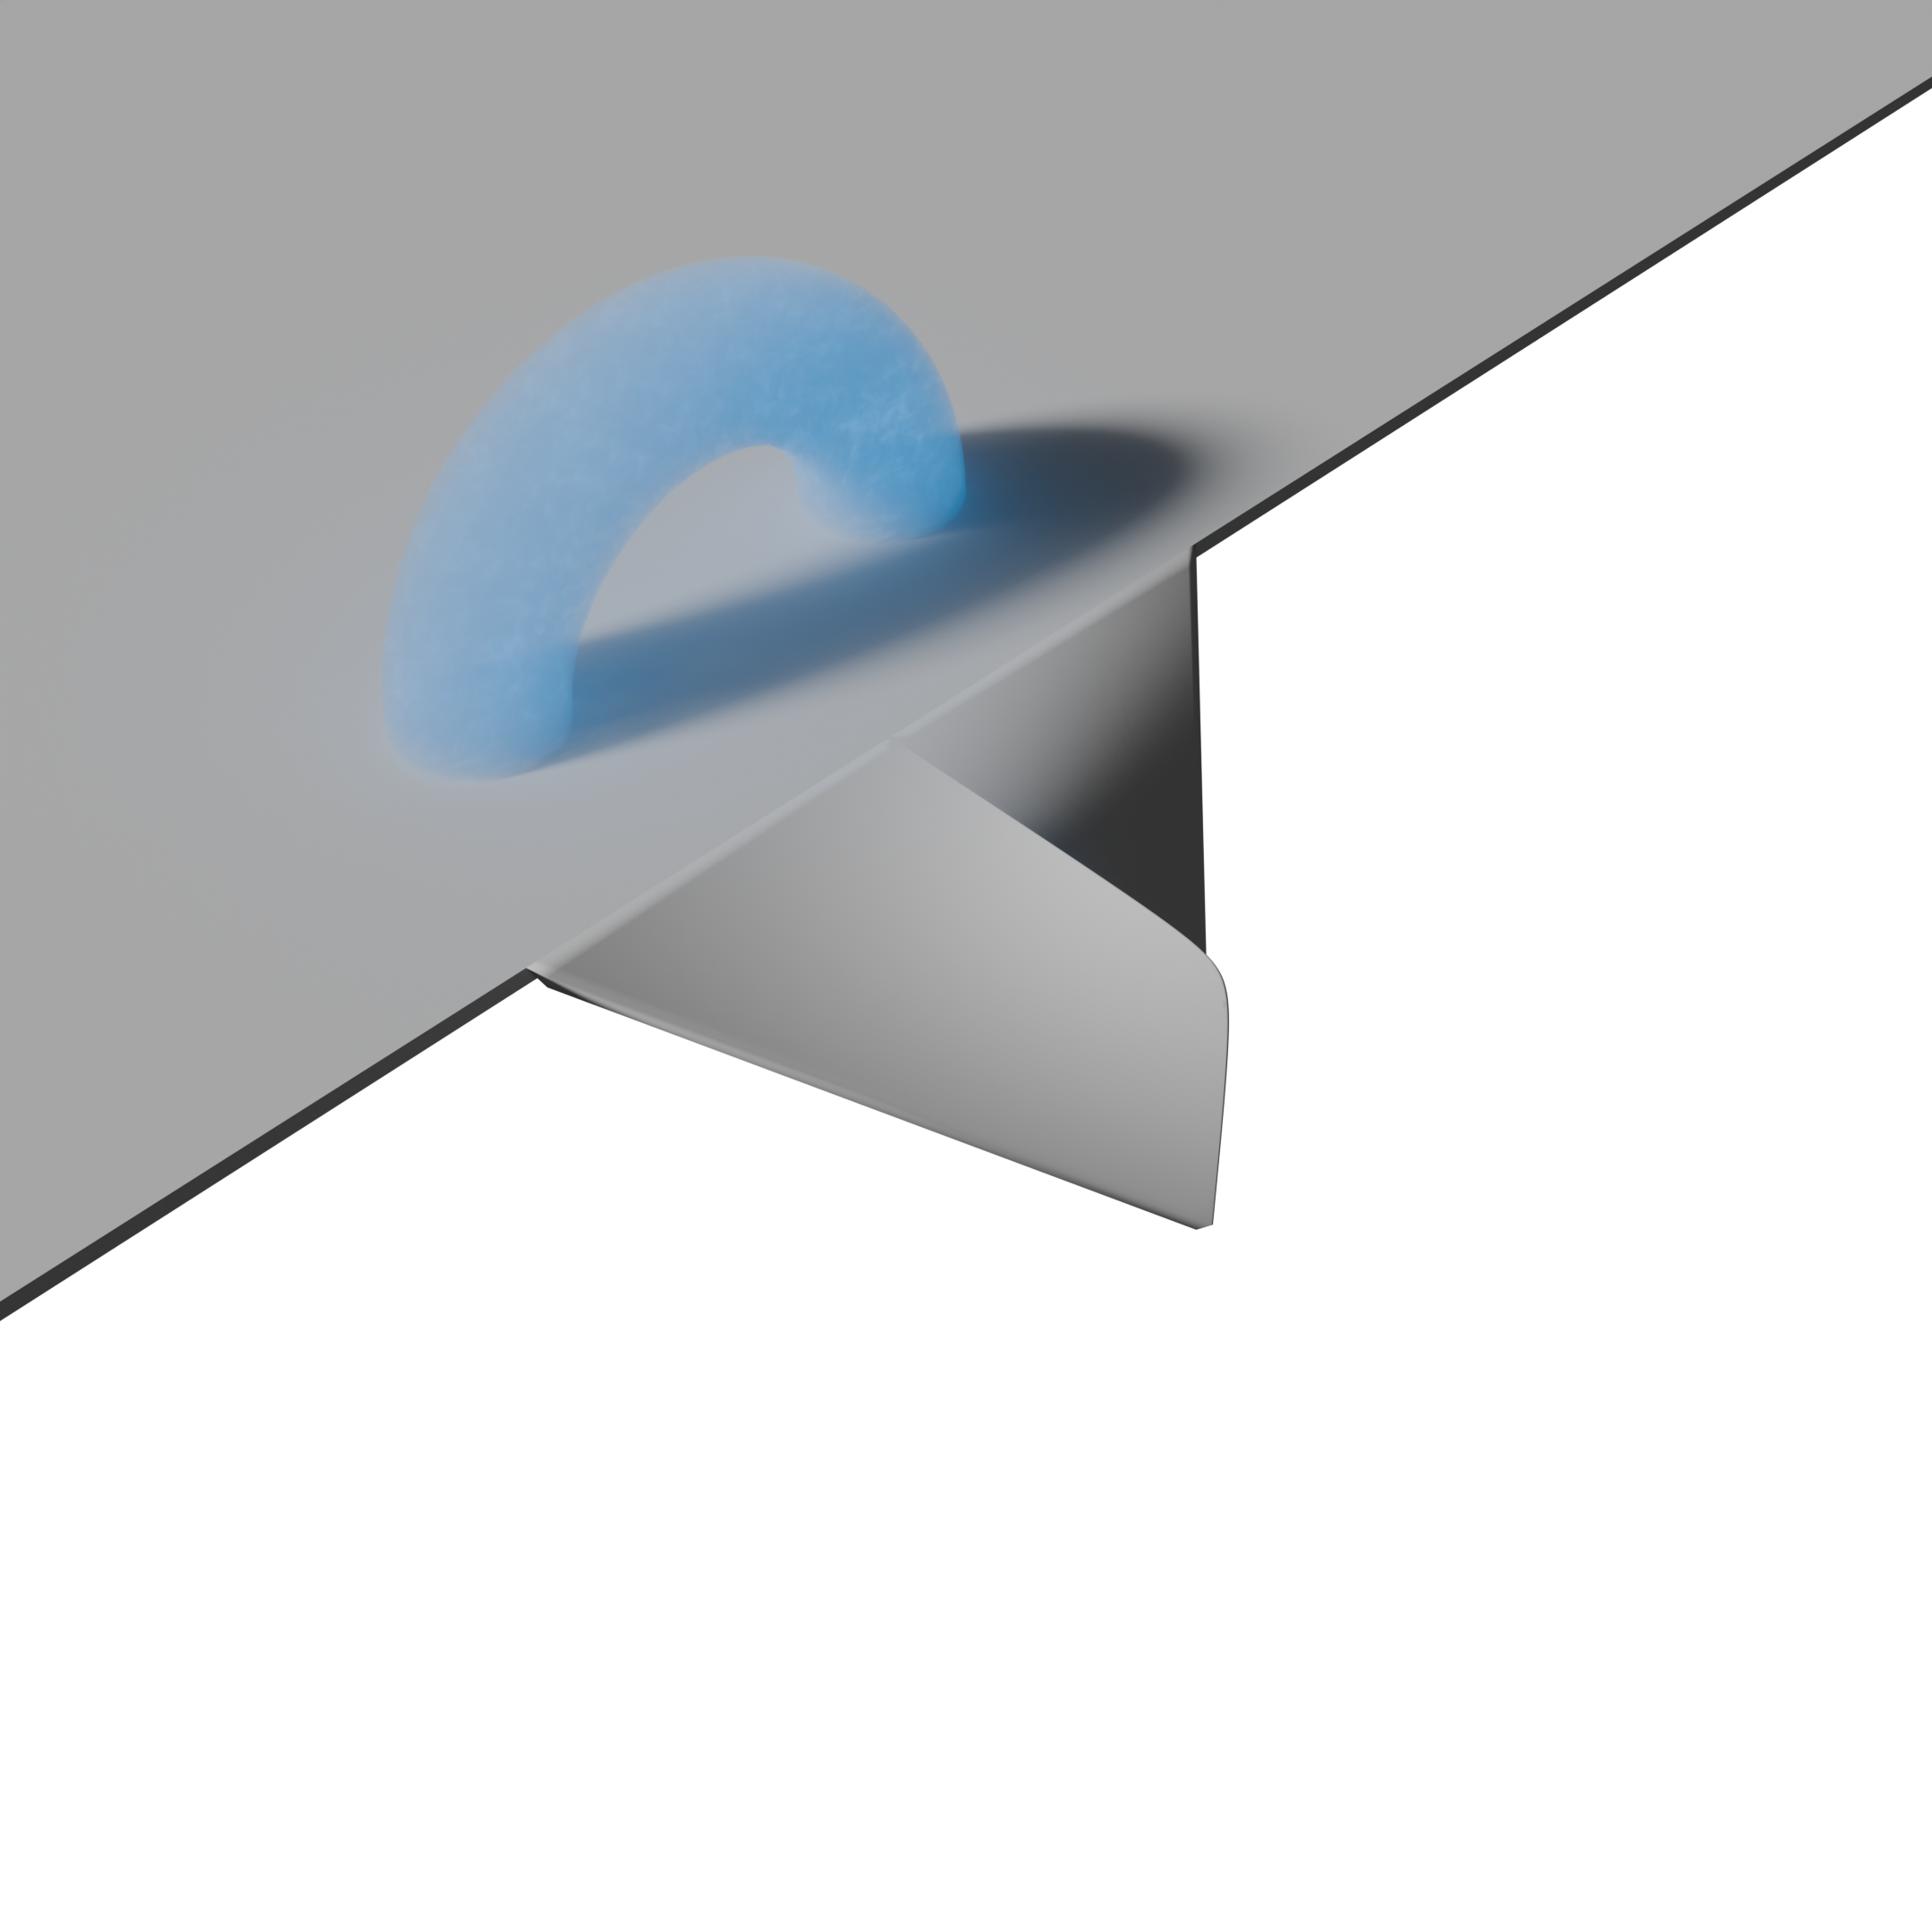
\includegraphics[width=0.3\textwidth]{papers/wirbelringe/fig/versuch_moment_3.png}
        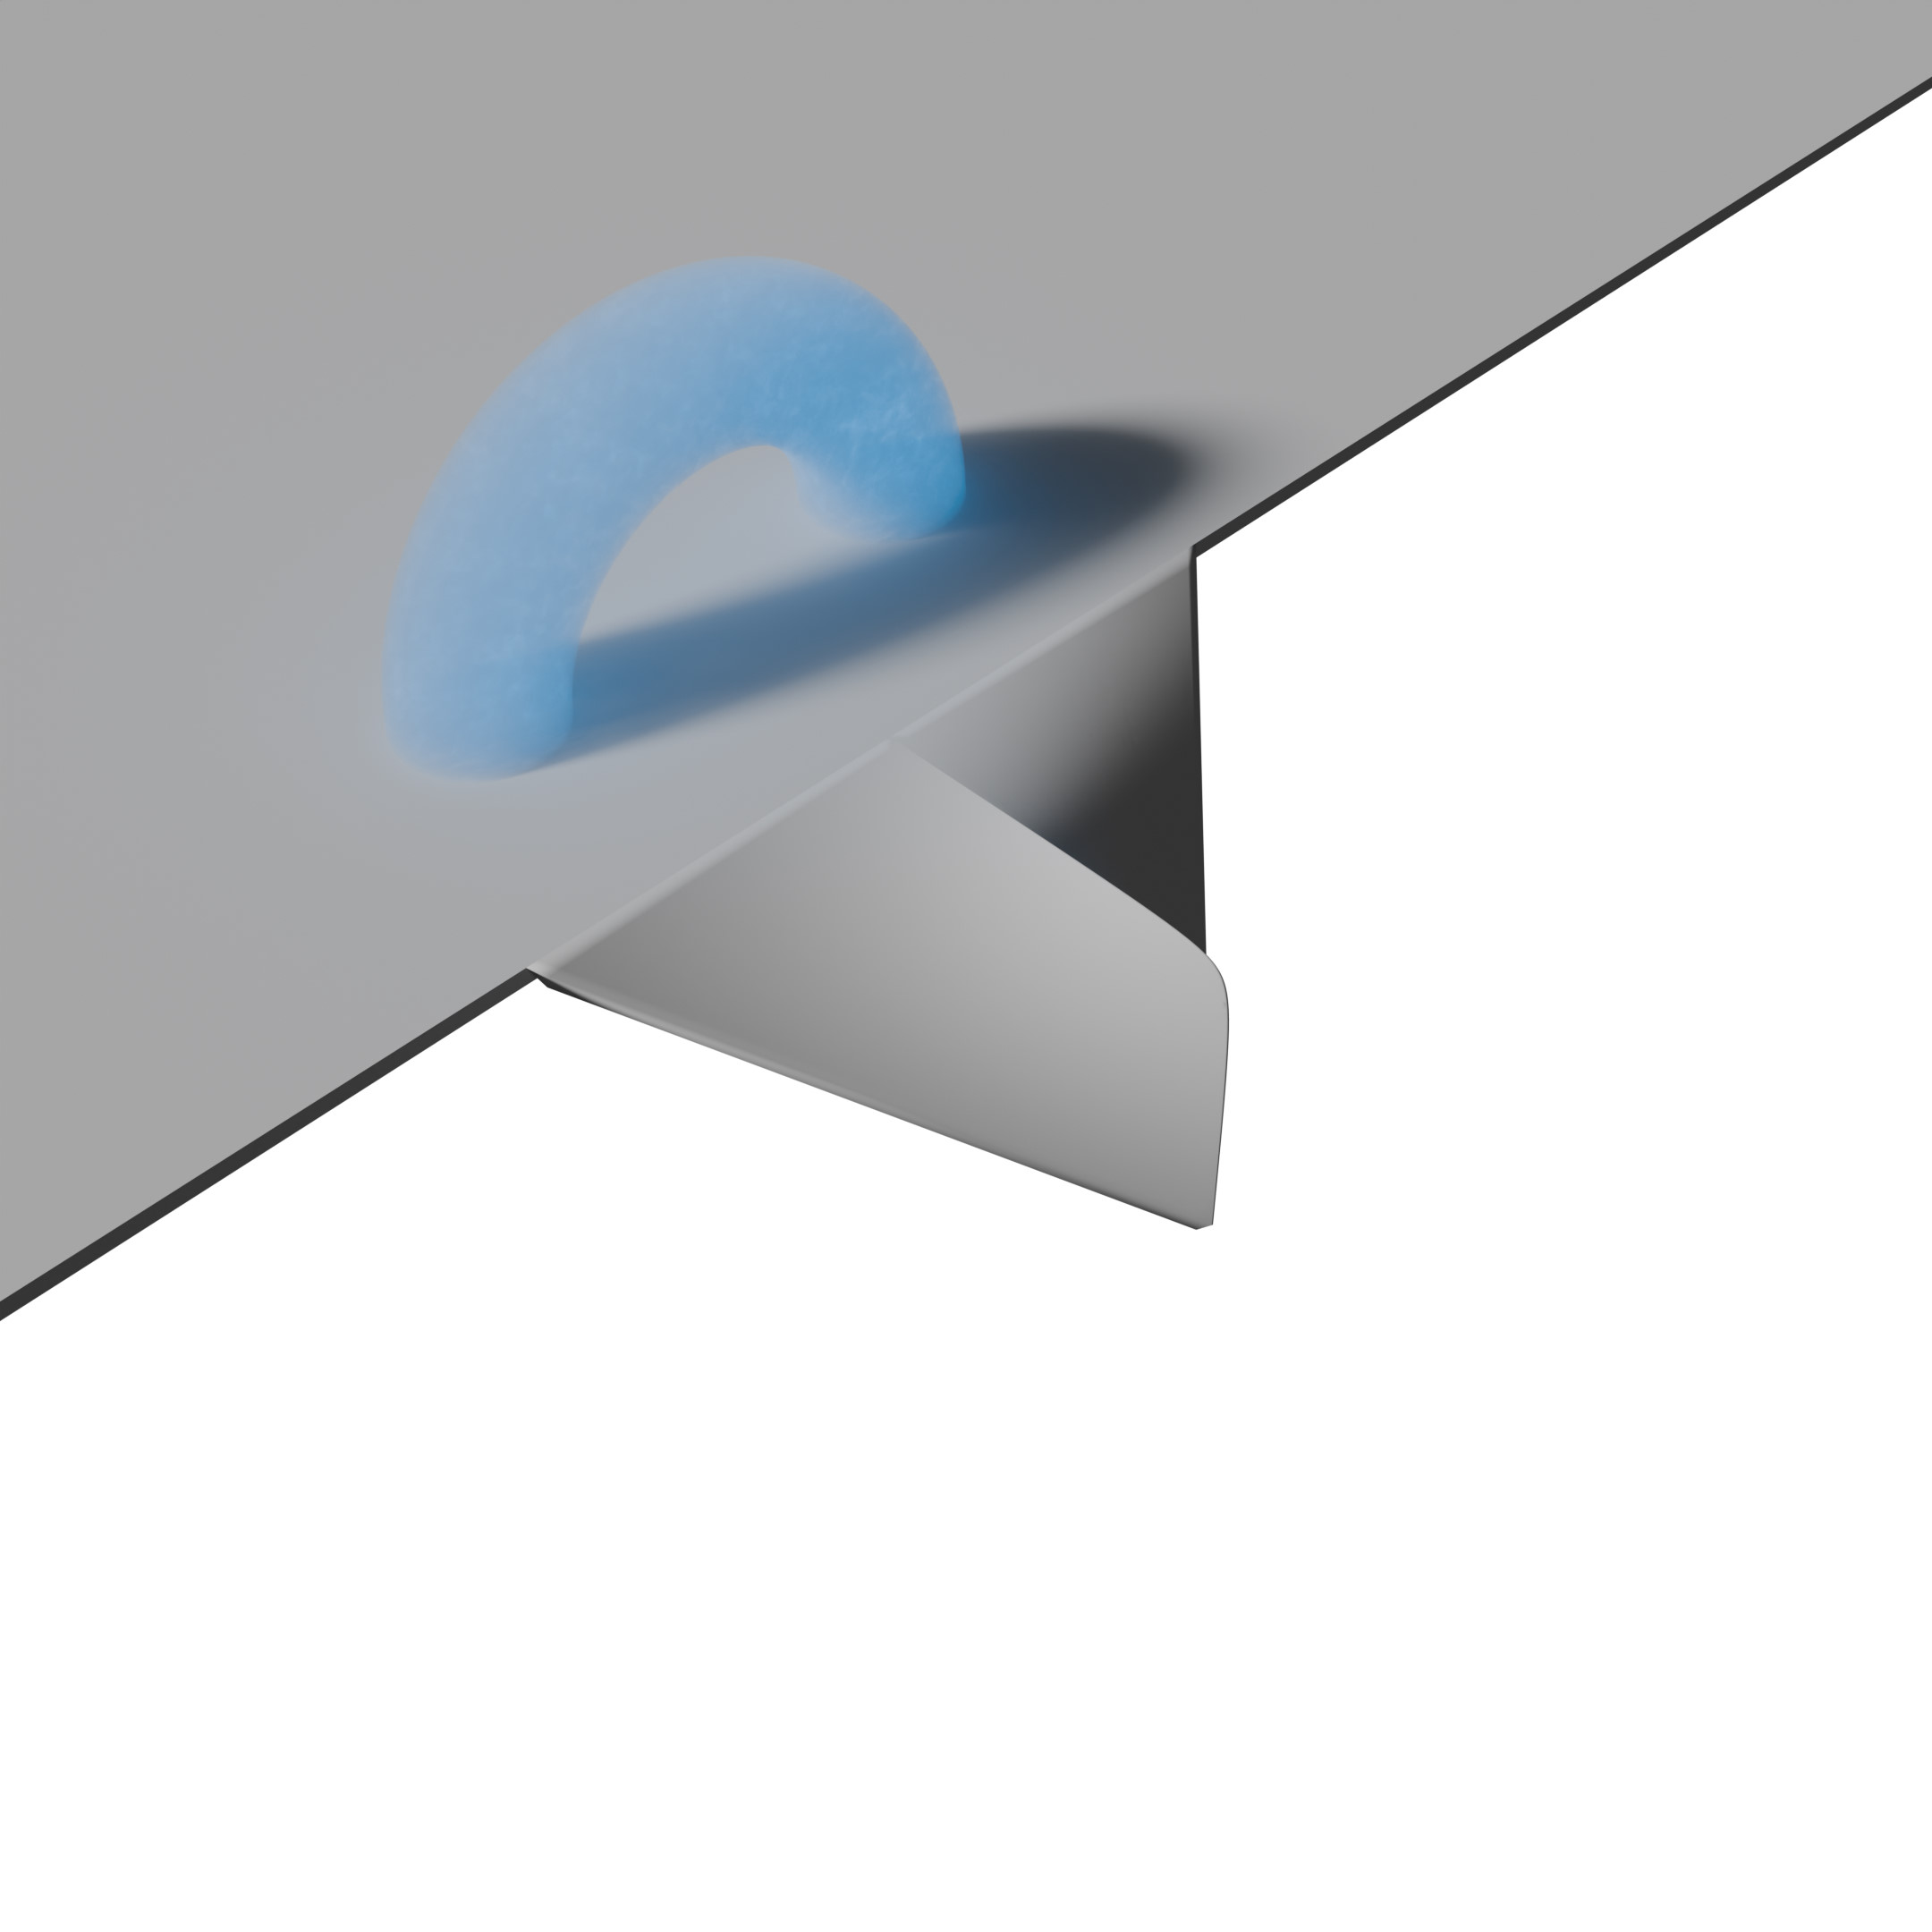
\includegraphics[width=0.3\textwidth]{papers/wirbelringe/fig/versuch_moment_3.jpg}
    }
    \caption{gewünschter Versuchsausgang}
    \label{buch:papers:Wirbelringe:fig:wirbelringversuch}
\end{figure}
